\section{Interaction Design}
\subsection{Usability Goals}
The below sections will be given points on a scale from 1 to 10, depending on
the importance (10 is very important and 1 is not important)
\begin{itemize}
	\item 10 safe to use (safety)
	\item 8 easy to learn (learnability) 
	\item 8 easy to remember how to use (memorability)
	\item 6 effective to use (effectiveness) 
	\item 5 efficient to use (efficiency/performance)
	\item 3 have good utility (utility)	
\end{itemize}
\subsubsection{Safety}
The safety is a very importanc factor, as the system is meant to placed outside
where some people might come by. Also the system is meant as a showoff system
for high-school students without any technically experience who might be
interrested in touching with everything possible.
\subsubsection{Learnability}
Should be easy to learn how to use, because\ldots
\subsubsection{Memoriability}
The system is build for Jan Nielsen who will probably only use the system when
people comes by and wants to see the system.
\subsubsection{Effectiveness}
The effectiveness of the system is not that important because\ldots
\subsubsection{Efficiency/Performance}
The efficiency of the system is not that important because\ldots
\subsubsection{Utility}
Not that important as it should be as simple as possible a system.
\subsection{User experience goals}
Down below the user experience goals are listed in nummeric order:
\begin{enumerate}
	\item Entertaining
	\item Motivating
	\item Satisfying
	\item Fun
	\item Enjoyable
	\item Helpful
	\item Aesthetically pleasing
	\item Supportive or creativity rewarding
	\item Emotionally fulfilling
	\item more?
\end{enumerate}
Something about why the list about looks like it does.

\begin{figure}[h!]		%Remember to put the h!, to not fuck the sections.
 \begin{centering}
  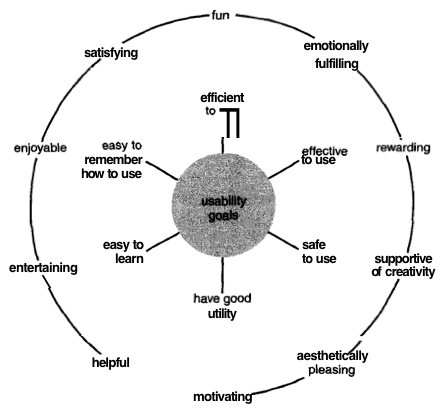
\includegraphics[width=0.5\textwidth]{images/usability_goals_diagram.png}
   \caption{Usability and user experience goals. Usability goals are central to
  			interaction design and are operationalized through specific criteria. 
  			User experience goals are shown in the outer circle and are less clearly defined.}
 \end{centering}
\end{figure}

This picture is taken direktly from the book, the caption too . Should it be
there ?
